%-----------------------------------------------------------------------
% Beginning of article.tex
%-----------------------------------------------------------------------
%
% AMS-LaTeX 1.2 sample file for book proceedings, based on amsproc.cls.
%
% Replace amsproc by the documentclass for the target series, e.g. pspum-l.amsfonts,amscd,amssymb,
%
%\documentclass{amsproc}
\documentclass[reqno,11pt]{amsart}
%\documentclass[10pt]{amsart}
\usepackage{epsfig,amscd,amssymb,amsmath,amsfonts}

%\usepackage{rotating}
%\usepackage{amssymb}
%\usepackage{epsfig}
\usepackage{amsmath}
\usepackage{graphicx}
\usepackage{amsthm,color}
\usepackage{tikz}
\usepackage{comment}
%\usetikzlibrary{graphdrawing.trees}
\usetikzlibrary{graphs}
\usetikzlibrary{graphs,quotes}
\usetikzlibrary{decorations.pathmorphing}

\tikzset{snake it/.style={decorate, decoration=snake}}
\tikzset{snake it/.style={decorate, decoration=snake}}

\usetikzlibrary{decorations.pathreplacing,decorations.markings,snakes}

\newtheorem{theorem}{Theorem}[section]
\newtheorem{lemma}[theorem]{Lemma}
\newtheorem{proposition}{Proposition}[section]
\theoremstyle{definition}
\newtheorem{definition}[theorem]{Definition}
\newtheorem{corollary}[theorem]{Corollary}
\newtheorem{conjecture}[theorem]{Conjecture}
\newtheorem{question}[theorem]{Question}
\newtheorem{example}[theorem]{Example}
\newtheorem{xca}[theorem]{Exercise}

\theoremstyle{remark}
\newtheorem{remark}[theorem]{Remark}

\numberwithin{equation}{section}

%    Absolute value notation
%\newcommand{\abs}[1]{\lvert#1\rvert}
%	 Shortcut for Exterior Notation
%	 	First entry for subscript
%		Second entry for number in "2(insert here) + 1"
%\newcommand{\exter}[2]{\Lambda^{S^2}_{#1}(2#2 + 1)}

\usepackage[margin=1.05in]{geometry}
\usepackage[colorlinks]{hyperref}
\usepackage{siunitx}









\makeatletter
\let\@wraptoccontribs\wraptoccontribs
\makeatother


%    Blank box placeholder for figures (to avoid requiring any
%    particular graphics capabilities for printing this document).

%\pagestyle{empty}
\begin{document}




\title[Twin-star hypothesis and cycle-free $d$-partitions of $K_{2d}$ ]{Twin-star hypothesis and cycle-free $d$-partitions of $K_{2d}$  }
%    Information for first author


\author{Matthew J. Fyfe }
\address{Department of Mathematics and Statistics, Bowling Green State University, Bowling Green, OH 43403 }
\email{mjfyfe@bgsu.edu}

% Information for second author

\author{Steven R. Lippold}
\address{Department of Chemistry, Mathematics, and Physics, Geneva College, Beaver Falls, PA 15010 }
\email{srlippol@geneva.edu}

%    Information for third author

\author{Mihai D. Staic}
%    Address of record for the research reported here
\address{Department of Mathematics and Statistics, Bowling Green State University, Bowling Green, OH 43403 }
\address{Institute of Mathematics of the Romanian Academy, PO.BOX 1-764, RO-70700 Bu\-cha\-rest, Romania.}

%    Current address
%\curraddr{}
\email{mstaic@bgsu.edu}


%	Information for fourth author

\author{Alin Stancu}
\address{Department of Mathematics, Columbus State  University, Columbus, GA 31907}
\email{stancu\_alin1@columbusstate.edu}

\maketitle


\section{Summary}
In this document we explain how one can use  MATLAB  to prove that the twin-star hypothesis $\mathcal{H}(4)$ holds true. This combined with a Theorem from the article ``Twin-Star Hypothesis and Cycle-Free $d$-Partitions of $K_{2d}$'' to show that a Conjecture from the same article is true for $d=4$. These results prove the twin-star hypothesis in this case. For more information on the Theorem and Conjecture in question, as well as the statement of the twin-star hypothesis, see the article cited.
\section{MATLAB Explanation}
\subsection{Initial Observations}
First, notice that from the article we know that in order to show that the twin-star hypothesis $\mathcal{TS}(4)$ holds true it is enough to show that very cycle-free $4$-partition of $K_8$ that contains the graph $T_{19}$ as one of its components is involution equivalent with a cycle-free $4$-partition of $K_8$ that contains the graph $TS_4$ as one of its components. 


Let $(\Gamma_1, \Gamma_2, \Gamma_3, \Gamma_4)$ be a cycle-free partition of $K_8$ such that one of the graphs $\Gamma_i$ is isomorphic to $T_{19}$. Using the action of $S_4$ on $\mathcal{P}_4^{cf}(K_8)$ we may assume that the cycle-free $4$-partition $(\Gamma_1, \Gamma_2, \Gamma_3, \Gamma_4)$ has the property that $\Gamma_1$ is isomorphic to $T_{19}$. Up to the $S_4$ action, this is equivalent to $\Gamma_4$ being isomorphic to $T_{19}$, as given in the article. However, it is more straightforward in the MATLAB code to take $\Gamma_1$ to be isomorphic to $T_{19}$.

Next, using the action of the group $S_8$ on on $\mathcal{P}_4^{cf}(K_8)$) (via the action on the vertices of $K_8$), we may assume that $E(\Gamma_1)=\{(1,2), (1,4), (1,6), (1,8), (2,3), (2,5), (4,7)\}$. Finally, since $(\Gamma_1, \Gamma_2, \Gamma_3, \Gamma_4)$ is cycle-free, the vertex $1$ must be incident to at least one edge of $\Gamma_i$ for all $1\leq i\leq 4$, so we may assume that $(1,3)\in E(\Gamma_2)$, $(1,5)\in E(\Gamma_3)$, and $(1,7)\in E(\Gamma_4)$ (here we use again the action of $S_4$ on $\mathcal{P}_4^{cf}(K_8)$).  A template for our partition is presented in Figure \ref{figtemplate}. 

\begin{figure}[h!]
	\centering
	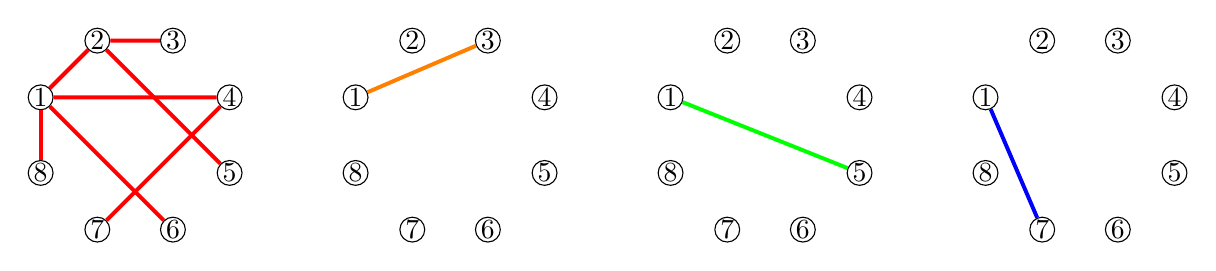
\begin{tikzpicture}
		[scale=0.8,auto=left,every node/.style={shape = circle, draw, fill = white,minimum size = 1pt, inner sep=0.3pt}]%baseline=(a.center)]%{circle,fill=black}]
		%\tikzset{VertexStyle/.style = {shape = circle,fill = black,minimum size = 9mm,inner sep=2pt}}
		\node (n1) at (0,2.1) {1};
		\node (n2) at (0.9,3)  {2};
		\node (n3) at (2.1,3)  {3};
		\node (n4) at (3,2.1)  {4};
		\node (n5) at (3,0.9)  {5};
		\node (n6) at (2.1,0)  {6};
		\node (n7) at (0.9,0)  {7};
		\node (n8) at (0,0.9)  {8};
		%\node (front) at (-2,0.5)   {$\Gamma_1$}
		\foreach \from/\to in {n1/n2,n1/n4,n1/n6,n1/n8,n2/n3,n2/n5,n4/n7}
		\draw[line width=0.5mm,red]  (\from) -- (\to);	
		\node (n12) at (5,2.1) {1};
		\node (n22) at (5.9,3)  {2};
		\node (n32) at (7.1,3)  {3};
		\node (n42) at (8,2.1)  {4};
		\node (n52) at (8,0.9)  {5};
		\node (n62) at (7.1,0)  {6};
		\node (n72) at (5.9,0)  {7};
		\node (n82) at (5,0.9)  {8};
		%\node (front) at (-2,0.5)   {$\Gamma_1$}
		\foreach \from/\to in {n12/n32}
		\draw[line width=0.5mm,orange]  (\from) -- (\to);	
		
		\node (n13) at (10,2.1) {1};
		\node (n23) at (10.9,3)  {2};
		\node (n33) at (12.1,3)  {3};
		\node (n43) at (13,2.1)  {4};
		\node (n53) at (13,0.9)  {5};
		\node (n63) at (12.1,0)  {6};
		\node (n73) at (10.9,0)  {7};
		\node (n83) at (10,0.9)  {8};
		%\node (front) at (-2,0.5)   {$\Gamma_1$}
		\foreach \from/\to in {n13/n53}
		\draw[line width=0.5mm,green]  (\from) -- (\to);	
		
		\node (n14) at (15,2.1) {1};
		\node (n24) at (15.9,3)  {2};
		\node (n34) at (17.1,3)  {3};
		\node (n44) at (18,2.1)  {4};
		\node (n54) at (18,0.9)  {5};
		\node (n64) at (17.1,0)  {6};
		\node (n74) at (15.9,0)  {7};
		\node (n84) at (15,0.9)  {8};
		%\node (front) at (-2,0.5)   {$\Gamma_1$}
		\foreach \from/\to in {n14/n74}
		\draw[line width=0.5mm,blue]  (\from) -- (\to);
		
		%\node[state,above of=B1] (C1) {$C_1$};
	\end{tikzpicture}
	\caption{ $\Gamma_1=X_{19}$, $(1,3)\in E(\Gamma_2)$, $(1,5)\in E(\Gamma_3)$, and $(1,7)\in E(\Gamma_4)$} \label{figtemplate}
\end{figure}

The plan is to analyze all cycle-free $4$-partitions of $K_8$ that have these properties and show that each such partition is involution equivalent with a cycle-free $4$-partition of $K_8$ that contains the graph $TS_4$ as one of its components. 

\subsection{Step 1: Generate Partitions}
Next we explain the MATLAB code that we developed to check this property. First we enumerate the edges of $K_8$ as follows: $(1,2)$ is the first edge, $(1,3)$ is the second, and so on with the edge $(7,8)$ being the  the $28$-th  (see the vector {\ttfamily AlphS2D4} in the file {\ttfamily  Step1GeneratePartitions.m}). With this convention, a homogeneous $4$-partition  $(\Gamma_1,\Gamma_2,\Gamma_3,\Gamma_4)$ of $K_8$ is described by a vector $v\in \mathbb{Z}^{28}$ whose entries are distinct values of the set $\{1,2,\dots,28\}$. The first seven entries of the vector $v$ correspond to $\Gamma_1$, the next seven to $\Gamma_2$, the next seven to $\Gamma_3$, and the last seven to $\Gamma_4$. In order to get a unique description of our partition we add the assumption that  $v(1)<v(2)<\dots<v(7)$, $v(8)<v(9)<\dots<v(14)$, $v(15)<v(16)<\dots<v(21)$, 
 and $v(22)<v(23)<\dots<v(28)$. 
For example,  the vector 
$$v=[1,2,4,6,9,11,13,3,8,14,15,17,20,22,5,10,16,19,23,24,27,7,12,18,21,25,26,28]$$ corresponds to the $4$-partition in Figure \ref{figd4}.

\begin{figure}[h!]
	\centering
	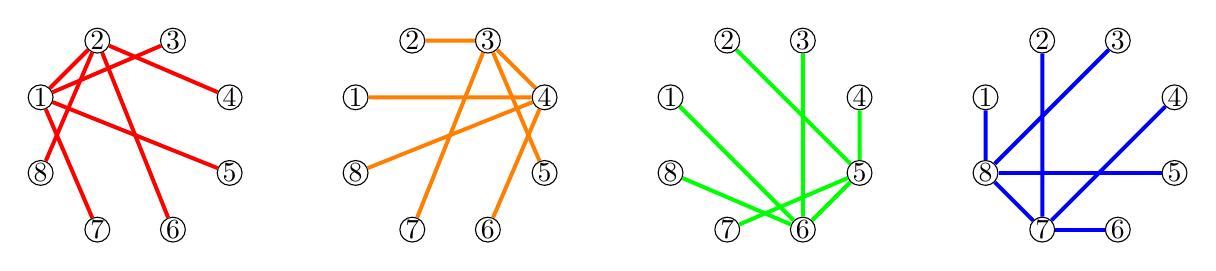
\begin{tikzpicture}
		[scale=0.8,auto=left,every node/.style={shape = circle, draw, fill = white,minimum size = 1pt, inner sep=0.3pt}]%baseline=(a.center)]%{circle,fill=black}]
		%\tikzset{VertexStyle/.style = {shape = circle,fill = black,minimum size = 9mm,inner sep=2pt}}
		\node (n1) at (0,2.1) {1};
		\node (n2) at (0.9,3)  {2};
		\node (n3) at (2.1,3)  {3};
		\node (n4) at (3,2.1)  {4};
		\node (n5) at (3,0.9)  {5};
		\node (n6) at (2.1,0)  {6};
		\node (n7) at (0.9,0)  {7};
		\node (n8) at (0,0.9)  {8};
		%\node (front) at (-2,0.5)   {$\Gamma_1$}
		\foreach \from/\to in {n1/n2,n1/n3,n1/n5,n1/n7,n2/n4,n2/n6,n2/n8}
		\draw[line width=0.5mm,red]  (\from) -- (\to);	
		\node (n12) at (5,2.1) {1};
		\node (n22) at (5.9,3)  {2};
		\node (n32) at (7.1,3)  {3};
		\node (n42) at (8,2.1)  {4};
		\node (n52) at (8,0.9)  {5};
		\node (n62) at (7.1,0)  {6};
		\node (n72) at (5.9,0)  {7};
		\node (n82) at (5,0.9)  {8};
		%\node (front) at (-2,0.5)   {$\Gamma_1$}
		\foreach \from/\to in {n32/n22,n32/n42,n32/n52,n32/n72,n42/n12,n42/n62,n42/n82}
		\draw[line width=0.5mm,orange]  (\from) -- (\to);	
		
		\node (n13) at (10,2.1) {1};
		\node (n23) at (10.9,3)  {2};
		\node (n33) at (12.1,3)  {3};
		\node (n43) at (13,2.1)  {4};
		\node (n53) at (13,0.9)  {5};
		\node (n63) at (12.1,0)  {6};
		\node (n73) at (10.9,0)  {7};
		\node (n83) at (10,0.9)  {8};
		%\node (front) at (-2,0.5)   {$\Gamma_1$}
		\foreach \from/\to in {n53/n63,n23/n53,n43/n53,n53/n73,n13/n63,n33/n63,n63/n83}
		\draw[line width=0.5mm,green]  (\from) -- (\to);	
		
		\node (n14) at (15,2.1) {1};
		\node (n24) at (15.9,3)  {2};
		\node (n34) at (17.1,3)  {3};
		\node (n44) at (18,2.1)  {4};
		\node (n54) at (18,0.9)  {5};
		\node (n64) at (17.1,0)  {6};
		\node (n74) at (15.9,0)  {7};
		\node (n84) at (15,0.9)  {8};
		%\node (front) at (-2,0.5)   {$\Gamma_1$}
		\foreach \from/\to in {n74/n84,n74/n24,n44/n74,n64/n74,n14/n84,n34/n84,n54/n84}
		\draw[line width=0.5mm,blue]  (\from) -- (\to);
		
		%\node[state,above of=B1] (C1) {$C_1$};
	\end{tikzpicture}
	\caption{A homogeneous cycle-free $4$-partition of  $K_8$ associated with the given vector} \label{figd4}
\end{figure}

With these conventions, we are looking for vectors $v\in \mathbb{Z}^{28}$ with the  $v(i)\in \{1,2,\dots,28\}$, $v(i)\neq v(j)$ if $i\neq j$, and $v(1)<v(2)<\dots<v(7)$, $v(8)<v(9)<\dots<v(14)$, $v(15)<v(16)<\dots<v(21)$, 
 and $v(22)<v(23)<\dots<v(28)$.  Moreover, since we fixed $\Gamma_1$ and the edges $(1,3)\in E(\Gamma_2)$, $(1,5)\in E(\Gamma_3)$, and $(1,7)\in E(\Gamma_4)$, we want  that $v(1)=1$, $v(2)=3$, $v(3)=5$, $v(4)=7$, $v(5)=8$, $v(6)=10$ and $v(7)=21$ (edges for $\Gamma_1$), $v(8)=2$ (because $(1,3)\in E(\Gamma_2)$),  $v(15)=4$ (because $(1,5)\in E(\Gamma_3)$), and $v(22)=6$ (because $(1,7)\in E(\Gamma_4)$). 


The first part of the code (file {\ttfamily Step1GeneratePartitions.m}) describes an algorithm that generates all cycle-free $4$-partitions with the above properties.  It turns out that there are \num{617088} such partitions.  The output of this search is the file {\ttfamily CycleFreePartitionsGamma1X19.txt}. This is primarily accomplished through empty arrays, the use of the nchoosek and setdiff functions in MATLAB, and with a user defined function that converts from the vector into a matrix that labels the edges.

\subsection{Step 2: Klein Group Action}


Next notice that the configuration in Figure \ref{figtemplate} is invariant under the action of a group isomorphic to the Klein group
$$K=\{e_{S_8}\times e_{S_4}, (6,8)\times e_{S_4}, (3,5)\times (2,3), (3,5)(6,8)\times (2,3)\}\subseteq S_8\times S_4$$

By use of this group action, we can reduce the number of partitions we need to examine by restricting ourselves to a representative of each of the equivalence classes. This is accomplished through the second part of code (file {\ttfamily Step2ActionKlein.m}), where we use this action to reduce the number of partitions we need to analyze. As expected, there are \num{154272} equivalence classes. The input is the file {\ttfamily CycleFreePartitionsGamma1X19.txt} and the output file is {\ttfamily CycleFreePartitionsKlein.txt}. 

\subsection{Step 3: Check for the twin-star graph}

The last part of the code (file {\ttfamily Step3CheckTS4.m}) shows that every partition from the file {\ttfamily CycleFreePartitionsKlein.txt} is at most three involutions away from a cycle-free $4$-partition that has one of the graphs isomorphic to $TS_4$. More precisely, for every $\mathcal{P}=(\Gamma_1, \Gamma_2, \Gamma_3,\Gamma_4)$ partition listed in {\ttfamily CycleFreePartitionsKlein.txt} there exist $1\leq a_i<b_i<c_i\leq 8$, for $1\leq i\leq 3$ such that if we denote 
\begin{eqnarray*}
\mathcal{P}_1&=&\mathcal{P}^{(a_1,b_1,c_1)},\\
\mathcal{P}_2&=&\mathcal{P}_1^{(a_2,b_2,c_2)},\\
\mathcal{P}_3&=&\mathcal{P}_2^{(a_3,b_3,c_3)},
\end{eqnarray*} 
then at least one of the cycle-free $4$-partition $\mathcal{P}_1$, $\mathcal{P}_2$,  or $\mathcal{P}_3$ contains a graph isomorphic to 
$TS_4$. 

\begin{remark} To check these results we used a PC with Core i7 processor, 12GB (RAM).  The run time was approximately  1.5 hours for the first file, 16 hours for the second, and 30 hours for the last.  With minimal modifications, one can skip the second file  (use only the first and the last file), but in that case the run time is about 120 hours. 
\end{remark}

\subsection{MATLAB Items}
Here is a short description of some of the main vectors, files, and functions used in our code.  For the complete MATLAB code see the Github Repository at https://github.com/Steven-R-Lippold/Twin-Star-Hypothesis.  
\begin{itemize}
\item the vector {\ttfamily  AlphS2D4} lists all edges in $K_8$. 
\item the file {\ttfamily CycleFreePartitionsGamma1X19.txt} gives a list of all cycle-free partitions with $E(\Gamma_1)=\{(1,2), (1,4), (1,6), (1,8), (2,3), (2,5), (4,7)\}$, $(1,3)\in \Gamma_2$, $(1,5)\in \Gamma_3$ and $(1,7)\in \Gamma_4$.
\item the function {\ttfamily Perm23(w28)} gives the action of the permutation $(2,3)\in S_4$ on the partition vector $w28\in \mathbb{Z}^{28}$. 
\item the function {\ttfamily sxw(sigma8,w28,AlphS2D4)} gives the action of the permutation $\sigma_8\in S_8$ on the partition vector $w28\in \mathbb{Z}^{28}$. 
\item the file {\ttfamily CycleFreePartitionsKlein.txt} gives a list of representatives for the action of the Klein group $K\in S_8\times S_4$ on the   cycle-free partitions from the file {\ttfamily CycleFreePartitionsGamma1X19.txt}.
\item the function {\ttfamily PartToVect(uu,AlphS2D4)},  associates to a $1\times 7$ vector $uu$ the corresponding matrix of edges.
\item the vector {\ttfamily AlphS2ABC} lists all triples $(a,b,c)$ with $1\leq a<b<c\leq 8$. 
\item {\ttfamily vHH=[4,4,1,1,1,1,1,1]} is the  incidence vector for the graph $TS_4$. 
\item the function {\ttfamily Step3DS(vxx,vHH,AlphS2D4,AlphS2ABC,rowsS2abc)} checks if the partition corresponding to $vxx$ is at most three involutions away from  a cycle-free $4$-partition which contains  a graph isomorphic to $TS_4$. 
\item the function {\ttfamily hasDS(txx,vHH,AlphS2D4)} decides if the cycle-free $4$-partition associated to the vector $txx$ contains a graph isomorphic to $TS_4$.
\item the function {\ttfamily ActABC(a,b,c,w28,AlphS2D4)} gives the action of the involution $(a,b,c)$ on the cycle-free $4$-partition associated to the vector $w28$. 
\item the file {\ttfamily NoPartitions.txt} list all partitions from {\ttfamily CycleFreePartitionsKlein.txt} that are not three involutions away from  a cycle-free $4$-partition which contains  a graph isomorphic to $TS_4$ (if our claim is correct, this file is empty). 
\end{itemize}

\end{document}

%-----------------------------------------------------------------------
% End of article.tex
%-----------------------------------------------------------------------

